\chapter{A Nossa Solução}
\label{sec:solucao}

Na Tarefa 1 começamos por contruir um tabuleiro com as mesmas dimensões do
caminho dado com somente com \texttt{Peca Lava 0}.

\begin{lstlisting}[language=Haskell]
 constroiTabuleiroBase :: Caminho -> Tabuleiro
\end{lstlisting}

Para isso usamos a função \texttt{dimensao}, definida pelos docentes, que nos dava
um par com a dimensão do tabuleiro para aquele caminho. Após contruir um
tabuleiro com essa dimensão, fomos substituindo as peças de lava pela a peça
imposta pelo caminho. Para isso foi preciso definir funções auxiliares que
tivessem em conta a altura das peças anteriores, a posição anterior e a
orientação.

Para validar os mapas gerados por caminhos, começamos por definir funções que
verificassem se cada uma das condições enunciadas na Secção
\ref{sec:analisefase1} eram respeitadas. Após isso, usamos a função final para
unir essas funções e descobrir se era ou não válido.

\begin{lstlisting}[language=Haskell]
 valida :: Mapa -> Bool
 valida (Mapa (p,o) tb) = a && b && c && d && e
                      where
                        a = orientacaoFstPeca (Mapa (p,o) tb)
                        b = periferiaLava tb
                        c = testaLava tb
                        d = testaPercurso (Mapa (p,o) tb)
                        e = verificaNotPercurso (Mapa (p,o) tb)
\end{lstlisting}

Na Tarefa 3 começamos por definir os casos em que o carro não morre. Desta
maneira conseguimos perceber que todos os casos restantes o carro morre e por
isso, a função movimenta deve retornar \texttt{Nothing}. Posto isto, tentamos
definir o caso mais simples em que não existe colisões que resultem em
ricochete, onde o movimento é linear, e devolver antes um carro em que a posição
foi correctamente alterada assim como o vetor velocidade possa ou não ter sido
alterado para refletir a mudança de direção do carro.

A Tarefa 4 tem o papel importante de definir o vetor velocidade consoante a ação
do jogador. Começamos por definir os vetores de todas as forças que atuam sobre
o carro separadamente. Com estas função definidas somavamos primeiro ao vetor
velocidade as forças da aceleração, do atrito, dos pneus e quando estava numa
rampa o vetor da gravidade. Nesse mesmo momento, a direção também era atualizada
quando o jogador estivesse a virar. Só depois disso é que aplicamos o vetor
nitro no caso de a ação do jogador assim o fizer. O vetor nitro é aplicado no
carro alvo, mas o tempo do histórico de nitro restante é retirado ao carro do
jogador. Nesta tarefa, uma vez que se tinha de atualizar todo o jogo, é também
atualizado o histórico de posições onde se acrescenta a posição atual à lista
caso esta ainda lá não esteja.

Na Tarefa 5 estabelecemos que iríamos definir a dimensão da janela do jogo como
(1000,1000) (pixeis). Deste modo, sabendo que as nossas imagens são quadradas e
têm 600 pixeis de lado, o próximo passo era definir um fator de scaling para as
imagens tendo em conta a dimensão do mapa que pretendemos desenhar.

Para conseguirmos desenhar um mapa precisamos de saber para que posições da
janela devem ir as peças, trabalho desempenhado pela função
\texttt{windowPositions}. Deste modo faltava associar peças a figuras, função
desempenhada pela função \texttt{pecaToPicture}. Deste modo, de forma sucinta, o
desenho de cada estado fica a cargo da função \texttt{drawState}.

\begin{figure}[h]
\label{fig:estado}
\centering
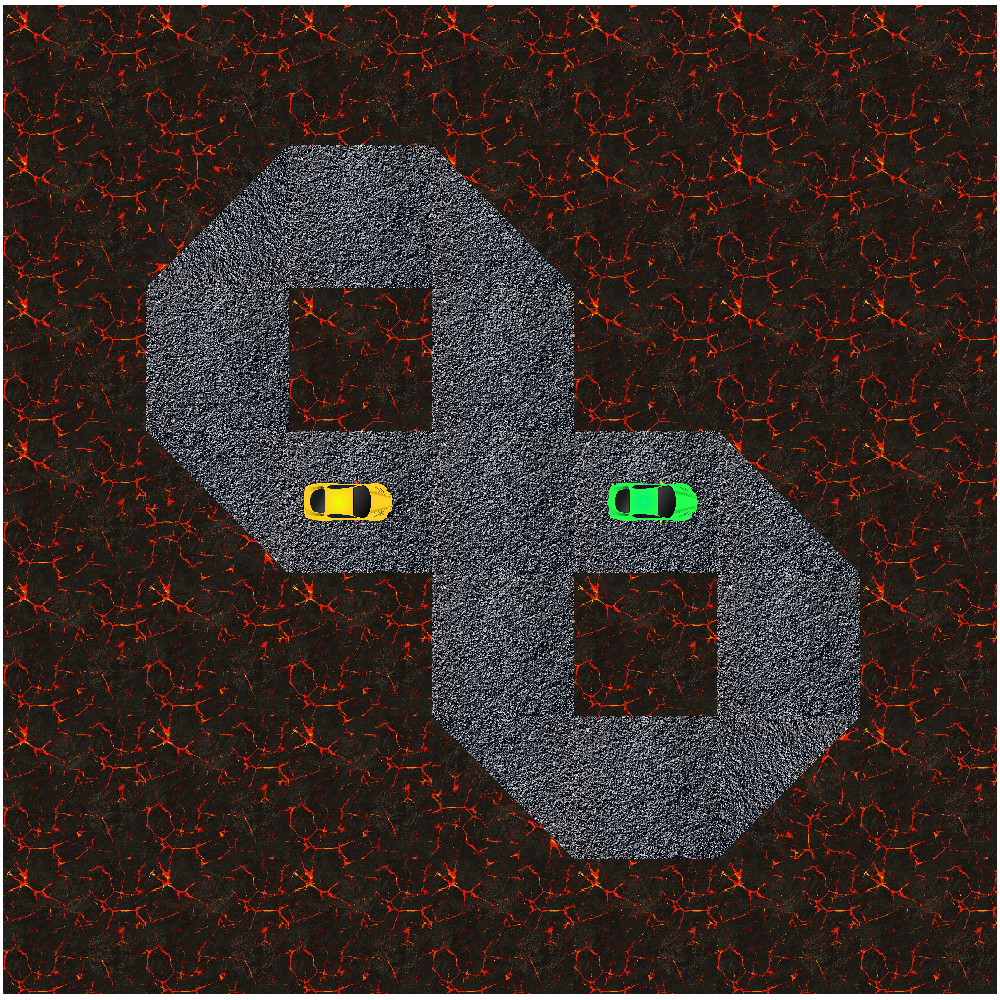
\includegraphics[width=8cm]{exemplo-mapa}
\caption{Exemplo de um estado do jogo.}
\end{figure}

Cada estado é constituído por uma lista de jogos, uma lista de imagens, uma
lista de ações, um bool e um inteiro. A lista de jogos contém os jogos
correspondentes aos quatros mapas do jogo em cada instante, as imagens são todas
as que foram carregadas em \texttt{main}, a lista de ações é constituída pela ação do
carro 1 e do carro 2 ou pela ação do carro 1 e ação do bot,
respetivamente. O bool é \texttt{False} caso a corrida ainda não tenha acabado e
\texttt{True} caso contrário. O inteiro identifica em que estado do jogo nos
encontramos.


Na Tarefa 6 para tentarmos alcançar o melhor resultado possível tentamos seguir
a seguinte estratégia:

\begin{itemize}
\item
  A base da estratégia é considerar a peça em que se está e a peça que
  vem a seguir.
\item
  Assim o bot analisa a peça em que se encontra e verifica a necessidade
  de virar para conseguir obter a direção necessária para que possa
  entrar corretamente na próxima peça.
\item
  A estratégia relativa à utilização de nitros passa essencialmente por
  verificar se o concorrente que se encontra mais próximo do nosso carro
  se encontra numa peça do tipo curva com altura superior ou igual a 0.
  Caso a condição anterior se verifique então aplicamos nitro ao
  concorrente, caso contrário apenas continuamos a marcha. Achamos
  pertinente incluir a claúsula relativa à altura porque na maioria dos
  casos se aplicassemos nitro a concorrente em peças do tipo curva com
  altura menor que 1 estes iriam ser ajudados ao invés de serem
  prejudicados em consequência das colisões que se verificam em peças
  com altura inferior a 0.
\end{itemize}
